


\documentclass[english,a4paper,babel,12pt]{nitathesis}

%%%%%%%%%%%%%%%%%%%%%%%%%%%%%%%%%%%%%%%%%%%%%

\usepackage{graphicx,times,epsfig,amsmath}
\usepackage[Sonny]{myfancy}
\usepackage{float}
\usepackage{xspace}
\usepackage{algorithmwh}
\usepackage{comment}
\usepackage{watermark}
\usepackage{graphicx}{\scriptsize {\footnotesize }}
\usepackage{pifont}
\usepackage{fancyhdr}
\usepackage{blindtext}


%%%%%%%%%%%%%%%%%%%%%%%%%%
\lhead{}
\chead{}
\rhead{CSED,NIT Agartala}
\lfoot{ }
\cfoot{\thepage}
\rfoot{}
%\setlength{\headrulewidth}{0.4pt}
%\setlength{\footrulewidth}{0.4pt}

\renewcommand{\headrulewidth}{0pt}
\renewcommand{\footrulewidth}{0.5pt}
%%%%%%%%%%%%%%%%%%%%%%%%%%



%\usepackage{algorithms}% \Add{} and \Del{} Corrections and \Mark{}
\begin{document}

% Using the watermark package which is in StyleFiles/
% and to remove DRAFT COPY ONLY appearing on the top of all pages comment out below line
%\watermark{SAMPLE COPY ONLY}






\beforepreface


\prefacesection{Acknowledgement}
I would like to take this opportunity to express my deep sense of gratitude to all who helped me directly or indirectly during this thesis work.
 I would like to thank my supervisor, \textbf{Ass. Prof. Mrs. Smita Das}, for being a great mentor and the best adviser, I could ever have. Her advise, encouragement and critics are source of innovative ideas, inspiration and causes behind the successful completion of this dissertation. The confidence shown on me  by her was the biggest source of inspiration 
for me. It has been a privilege working with her from last one year.\

I am highly obliged to all the faculty members of Computer Science and Engineering Department for their support and encouragement. 
I also thank our Director \textbf{Prof.(Dr.)~ H. K. Sharma} and H.O.D, CSED \textbf {Prof. (Dr.)~ Debasish Bhattacharya }
for providing excellent computing and other facilities without which this work could not achieve its quality goal.
\
 

 Finally, I am grateful to my \textbf{parents} for their support. It was impossible for me to complete 
this thesis work without their love, blessing  and
encouragement.
\\

\vspace*{0.5cm} \hspace*{11cm}\textbf{\large - Santosh Kumar}
\setcounter{page}{6}
 

\begin{comment}
 




\prefacesection{Biographical Sketch}

\begin{center}
{\textbf{\LARGE Prveen Kumar}}\end{center} \hrule
\begin{center}
412, Madhya Banamalipur  PIN-799001,  E-Mail: prveen.mnnit@gmail.com,  Contact. No. 09452987917 \\
 \end{center}

\subsection*{\textbf{Education}} 
\begin{itemize}
\item Pursuing M.Tech. in Computer Sc. \& Engg. branch from N.I.T,Agartala with CPI of 8.34/10/00.
\item B.Tech. in Information Technology branch from B.B.D.N.I.T.M. Lucknow with 70.82\% in 2008.
\item Intermediate from S.S.D.Inter College, Hasanpur with 66.2\% in 2002.
\item High School from Saraswati Vidya Mandir, Hasanpur with 71.00 \% in 2000.
\end{itemize}

\subsection*{\textbf{M.Tech Thesis Research Orientation}} 
IEEE LTSA framework has been able to genrate interest for implementation of e-Learning technology meant for two-tier or three tier.
 Such e-Learning framework lacks security aspect making it insufficient for web educational services through Service Oriented Architecture (SOA). Implementation of different security services at different
layers requires a pragmatic mapping from client-server architecture to distributed system architecture and finally to Service Oriented Architecture.

\subsection*{Publications}
\begin{enumerate}
 \item  Kumar, Prveen., Samaddar, Shefalika Ghosh., Samaddar, Arun B. \& Misra, Arun K., (2010); \textbf{Extending IEEE LTSA e­learning Framework in Secured SOA Environment}, 
  The 2nd IEEE International Conference on Education Technology and Computer (ICETC 2010), IEEE Education Society (ISBN: 978-1-4244-6368-8), Shanghai China, June 22-­24, 2010. 
\textbf{(Accepted)}
\item   Kumar, Prveen., Samaddar, Shefalika Ghosh., Samaddar, Arun B. \& Misra, Arun K.,(2010);\textbf{Extending IEEE LTSA e­learning Framework in Secured SOA Environment}, 
  IEEE Transaction on Leatning Technology. \textbf{(Under Peer Review)}

\end{enumerate}
\end{comment}


\prefacesection{Dedicated to}

\begin{center}
\vspace*{4cm}
\textit{ \textbf {To My Loving Family for their kind love \& support.\\
To my thesis supervisor Ass. Prof.~ Mrs. Smita Das for sharing her valuable knowledge,
 encouragement \& showing confidence on me all the time.
}} \end{center}

\newpage
\vspace*{6cm}
\textit{\textbf { \begin{large} \ding{125}You can't teach people everything they need to know. 
The best you can do is position them where they can find what they need 
to know when they need to know it.\ding{126}\end{large}}}\\
\vspace*{4cm} \hspace*{6.5cm} \textbf{-Seymour Paper (MIT Mathematician)} 

\prefacesection{Abstract}
The Banking System forms the core of the Financial Sector of any economy. The role of Commercial Banks is more relevant in developing economies.The future reform process need to be designed so that it should focus on ensuring sustained viability and efficiency of the Banking System. A leading banking  and credit card services provider \textbf {CORPORATION BANK} is trying to use Hadoop technologies to handle and analyze large amounts of data.
Currently, the organization has data in RDBMS but want to use the Hadoop ecosystem for storage, archival, and analysis of large amount of
data.
   %Producing 'blind' text for testing.




\afterpreface
\pagenumbering{roman}                     
\setcounter{page}{15}
%\listoffigures
%\pagenumbering{roman}
%\setcounter{page}{11}
\newpage
\pagenumbering{arabic}
\setcounter{page}{1}   


\pagestyle{fancy}

\flushbottom

\chapter{Introduction}
Banking system is an integral part of our society now a days.
Almost every working and nonworking individual need loan at some point of time.
So it is very important for the bank also to keep a check on weather the loans installments are being paid on time or not.
This application has been develops keeping in mind the above points.
The application provides for generation of a list of customers who have 2 or more than  loans in their name.
The application also provides for generation of a list of customers who have not paid the lone installment on the due date. \newline
In this project we can analysing the Banking System,like Loan\_information,Credit\_card\_info-        rmation and Shared\_information . So in this case all data is being analysed using Big Data and Hadoop tools. 


\flushbottom

\flushbottom
\chapter{Tools}

\subsection{Big Data}
Big Data is a phrase used to mean a massive volume of both structured and unstructured data that is so large it is difficult to process using traditional database and software techniques. In most enterprise scenarios the volume of data is too big or it moves too fast or it exceeds current processing capacity.

\section{Hadoop}
Hadoop is an open source distributed processing framework that manages data processing and storage for big data applications running in clustered systems.It is at the center of a growing ecosystem of big data technologies that are primarily used to support advanced analytics initiatives, including predictive analytics, data mining and machine learning applications. Hadoop can handle various forms of structured and unstructured data, giving users more flexibility for collecting, processing and analyzing data than relational databases and data warehouses provide.


\subsubsection{Single Node} 
Single node cluster means only one Data Node running and setting up all the Name Node, Data Node, Resource Manager and Node Manager on a single machine. This is used for studying and testing purposes. For example, let us consider a sample data set inside a healthcare industry. So, for testing whether the Oozie jobs have scheduled all the processes like collecting, aggregating, storing and processing the data in a proper sequence, we use single node cluster. It can easily and efficiently test the sequential workflow in a smaller environment as compared to large environments which contains terabytes of data distributed across hundreds of machines. 
\subsubsection{Multi Node} 
While in a Multi node cluster, there are more than one Data Node running and each Data Node is running on different machines. The multi node cluster is practically used in organizations for analyzing Big Data. Considering the above example, in real time when we deal with petabytes of data, it needs to be distributed across hundreds of machines to be processed. Thus, here we use multi node cluster.

\subsection{Pig }
Pig is a high-level programming language useful for analyzing large data sets. A pig was a result of development effort at Yahoo!.
In a Map Reduce framework, programs need to be translated into a series of Map and Reduce stages. However, this is not a programming model which data analysts are familiar with. So, in order to bridge this gap, an abstraction called Pig was built on top of Hadoop.

Apache Pig enables people to focus more on analyzing bulk data sets and to spend less time writing Map-Reduce programs. Similar to Pigs, who eat anything, the Pig programming language is designed to work upon any kind of data. That's why the name, Pig! 

\subsection{Sqoop }
Sqoop is a tool designed to transfer data between Hadoop and relational database servers. It is used to import data from relational databases such as MySQL, Oracle to Hadoop HDFS, and export from Hadoop file system to relational databases.
\subsection{HIVE}
Apache Hive is a data warehouse software project built on top of Apache Hadoop for providing data query and analysis. Hive gives a SQL-like interface to query data stored in various databases and file systems that integrate with Hadoop.
\section{Big Bank, Big Problem}
A leading banking and credit card services provider is trying to use Hadoop
technologies to handle and analyze large amounts of data.\newline
Currently, the organization has data in the RDBMS but wants to use the
Hadoop ecosystem for storage, archival, and analysis of large amounts of
data.
\section{Creating the Hadoop Cluster and Deploying Test Codes}
For any Big Data project, a proper environmental setup is mandatory. In
real world scenarios, a Hadoop cluster can consist of 40K clusters/nodes.
As it is not possible for us to build such a huge setup in an academic lab,
we will be going with minimal 2 node cluster and simulate the ingestion,
cleaning, analysis and send the report to the downstream team.
Create a Pseudo-Distributed Node Cluster and deploy all the test codes
using Maven and SBT.\newpage
\subsection{Data Ingestion}
Bring data from RDBMS to HDFS. This data import must be incremental
and should happen every 2 minutes.
\newline
Following tables have to be imported:
\begin{figure}[H]
\centering
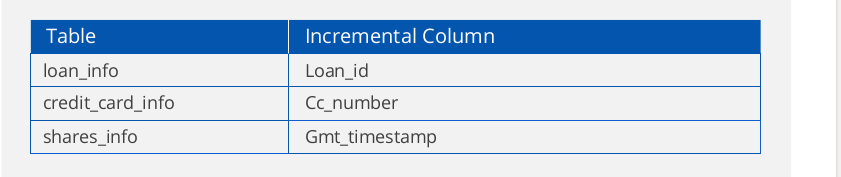
\includegraphics[width=12cm,height=3cm]{dataingestion.png}
    \caption{Data Ingestion}
\end{figure}
\newline
All these data must be encrypted in HDFS. The HDFS data should be
compressed to store less volume.\newline
The Sqoop password must also be encrypted.
\newline
Table Details:
\subsection{Loan\_info}
This table has following columns:\newline
\begin{figure}[H]
\centering
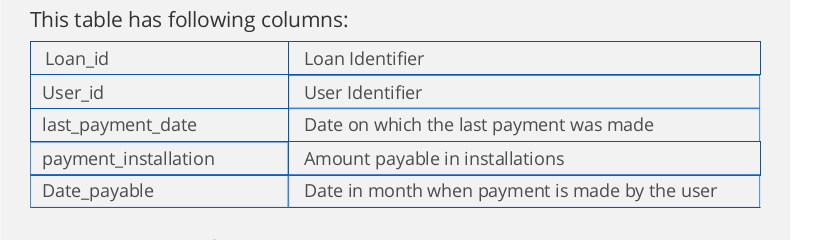
\includegraphics[width=12cm,height=3cm]{loan_info.png}
    \caption{Loan\_info}
\end{figure}\newpage
\subsection{Credit\_card\_info}
This table has the following columns:
\begin{figure}[H]
\centering
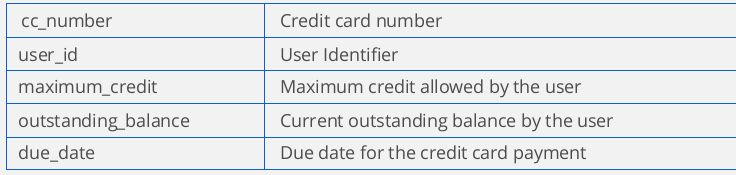
\includegraphics[width=12cm,height=3cm]{creditcard1.png}
    \caption{Credit\_card\_info}
\end{figure}
\newline
\subsection{Shares\_info}
This table has the following information:
\begin{figure}[H]
\centering
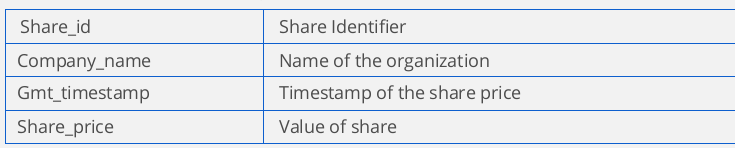
\includegraphics[width=12cm,height=3cm]{sharesinfo1.png}
    \caption{Shares\_info}
\end{figure}
\newline
\subsection{Analysis}
\item Find out the list of users who have at least 2 loan installments pending.
\item Find the list of users who have a healthy credit card but outstanding loan
account.
\items Healthy credit card means no outstanding balance.
\newline For every share and for every date, find the maximum profit one could
have made on the share. Bear in mind that a share purchase must be
before share sell and if share prices fall throughout the day, maximum
possible profit may be negative. \newpage
\subsection{Archival}
The organization has a lot of survey data scattered across different files in
a directory in local file system. Provide a mechanism to effectively store the
small files in Hadoop. It is expected to pack small files together before
actually storing them in HDFS.\newline
Survey files have the following structure:
\begin{figure}[H]
\centering
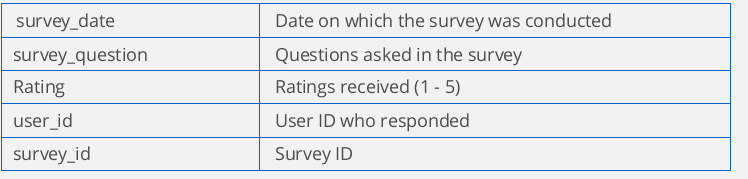
\includegraphics[width=12cm,height=3cm]{surveyfile.png}
    \caption{Survey files}
\end{figure}
\newpage











%The five different levels of the architecture represent the different points of view of
%%\begin{itemize}
% \item \textit{Layer 1}: This level defines the tasks of acquisition, transfer, exchange and
%discovery for the learner as a result of the interactions with his environment. The
%level is seen as two systems exchanging information.
 %\item \textit{Layer 2}: This layer defines the learner’s reaction to the environment. The
%definition is based on the specific design features of learner related modules.
  %\item \textit{Layer 3}: A component system, normalized by IEEE, defines an organization
%of a learning process, seen from the data and control flow point of view.
%  \item \textit{Layer 4}: This level exploits the component %system, directly, in order to
%formalize the technological design constraints. It allows the identification of the
%system’s activities during the learning process. This provides the genric views of
%all the stakeholders and therefore, takes care of their interest.
 % \item \textit{Layer 5}:  \blindtext
%\end{itemize}
%\begin{comment}
%\begin{figure}[htb]
 %\centering
 %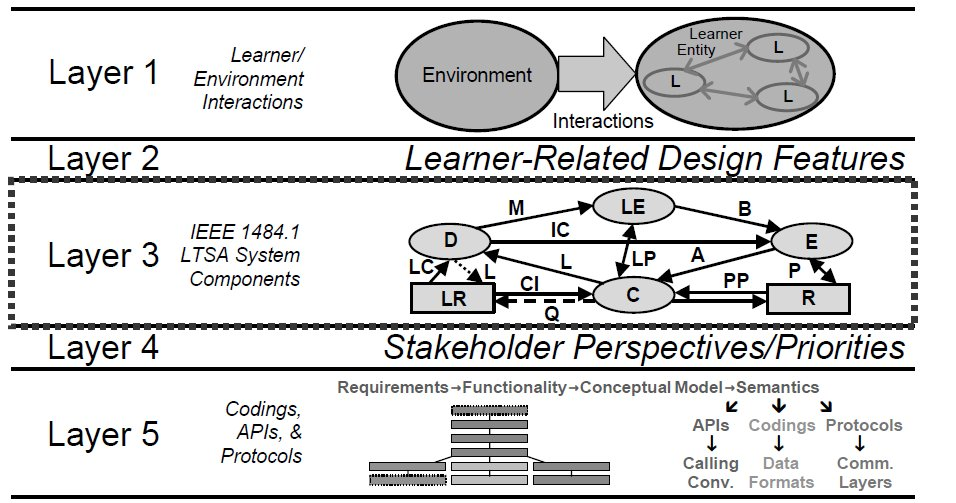
\includegraphics[scale=.4]{m.jpg}
 % m.jpg: 956x503 pixel, 72dpi, 33.73x17.74 cm, bb=0 0 956 503
% \caption{IEEE LTSA Layered Structure\cite{ltsa}}
%\end{figure}
%\end{comment}
%\subsection{A detailed description of LTSA system components at level 3}
% \blindtext types used are \cite{ltsa} (figure.2):
%\begin{enumerate}
 %\item \textit{The interaction context:} This flow of data gives the necessary information for
  %  interpretation of the observations.
%\item \textit{The observations:} This represents the real-time unabridged information concerning the learner activities.
%\item \textit{The acquisition state:} The evaluating process can send or update a learner profile (e.g. a response to a correct answer within a given time).
%\item \textit{The learner profile:} The tutoring process can %consult and modify learner information during the apprenticeship. This is a data-store
   % which updates the learner profile as per data-base management system dictat.
%\item \textit{The evaluation:} It informs the tutoring process of the present state of the
   % learner profile so as to optimize the learning process.
%\begin{comment}
%\begin{figure}[htb]
 %\centering
 %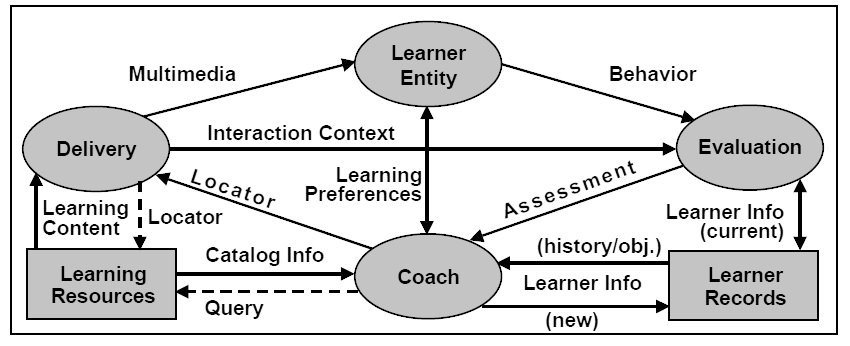
\includegraphics[scale=.6]{rj.jpg}
 % rj.jpg: 850x346 pixel, 72dpi, 29.99x12.21 cm, bb=0 0 850 346
% \caption{IEEE LTSA Layer-3 (System Components)\cite{ltsa}}
%\end{figure}
%\end{comment}
%\item  \textit{The learner preferences:} The tutoring process negotiates the teaching parameters with the learning actor(s).
%\item  \textit{The multimedia data:} This flow of data allows the learning process to use simultaneous pedagogical multimedia resources such as video, audio, text and
   % graphics. All these contents are devloped and designed as per scheme of e-Learning.
%\item  \textit{The locality:} This data or control flow indicates where to find a given pedagogical resource.
%\item  \textit{The pedagogical contents:} This data flow has the coded pedagogical material. The content presentation, in an appropriate format, is an
 %   outcome of this data flow.
%\item  \textit{The catalogued inquiries and information:} The tutoring process can carry out
 %   simple requests to find appropriate learning objects for a course. These requests
  %  may contain search criteria based on the learner’s preferences, the evaluation
   % results and the course information.

%\end{enumerate}  The role and the behavior of the different components are described using a
%learner scenario, which is divided into eight identified scenarios:
%\begin{enumerate}
 %\item The teaching style, the pedagogical choices and the acquisition methods are
%negotiated with the learner.
%\item The learning process is observed and evaluated in a context of action and
%interaction with the system.
%\item The evaluating process gives observations and indications about the learner
%style and/or information about the functioning /the state of the system.
%\item This data is stored in a data bank dedicated to the learner.
%\item The tutoring process analyses the learner’s performance from his assessments,
%his preferences, his past history and his future perspectives.
%\item This same process searches for suitable learning object using resource bank
%requests.
%\item The tutoring process extracts the pedagogical content from the proposed
%resources. It transmits the resource references to the diffusion process, organizing
%them, for example, into a pedagogical sequence.
%\item The diffusion process extracts the pedagogical contents %from the learning
%object to adapt it to the surrounding interface used by the learner.

%\end{enumerate}

%\subsection{Limitations of LTSA for e-Learning services}
%Some of the functional areas, that is not included in LTSA, are identified :
%\begin{itemize}
 %\item The model does not regard the learning object designer as an integrated
%component in the learning process.
 %\item The students evaluation records are stored but, the use is not specified. This
%brings ambiguity in case of e-Learning services to be provided and e-Learning services to be received to give services. 
%The composition of services becomes difficult.
 %\item For a distance mode learner, if the learner possesses some wrong/incomplete
%idea at the start and the feedback system fails to identify it, then the LTSA layer
%2 algorithm falls apart under a never ending iterative cycle. The learner can never
%be sure, that his learning activities are properly registered. Moreover, the system
%never recognizes the incomplete feedback or shows the partial data that may have
%been registered for the future use.
 %\item Students counseling is not included in the LTSA architecture. Students enrol

\flushbottom

\flushbottom
\chapter{Project Definition}
\subsection{Loading data into mysql}
\begin{figure}[H]
\centering
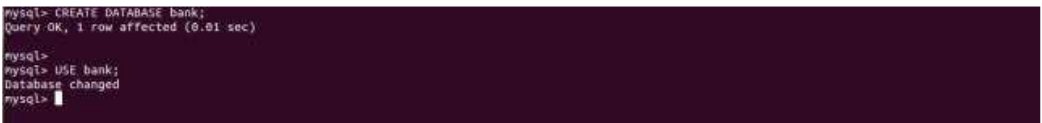
\includegraphics[width=12cm,height=3cm]{1.png}
    \caption{Database Name}
\end{figure}
 
 \section{Creating database bank in mysql:-}
 CREATE DATABASE bank; \newline
 USE bank;

 \newpage
 \section{Creating tables in mysql and inserting the data into mysql tables :-}
 \subsection{Creating table loan\_info}
 CREATE TABLE loan info (loan\_id int,user\_id int,last\_payment\_date DATE,payment\_installation DOUBLE,date\_payable DATE);
 
\begin{figure}[H]
\centering
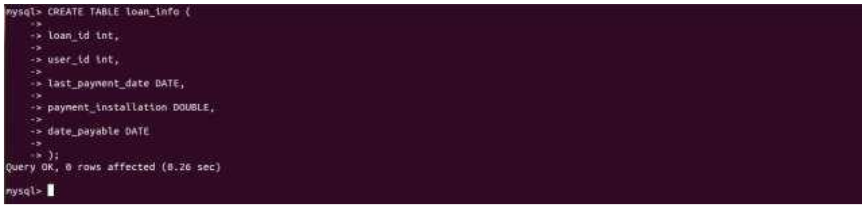
\includegraphics[width=12cm,height=3cm]{table2.png}
    \caption{loan\_info}
\end{figure}

\subsection{Inserting data into loan\_info table}
insert into loan\_info values(1234,5678,'2017-02-20',509,'2017-03-20');\newline
insert into loan\_info values(1243,5687,'2016-02-18',9087,'2016-03-18');\newline
insert into loan\_info values(1324,5786,'2017-03-01',8976,'2017-04-01');\newline
insert into loan\_info values(4312,8976,'2017-01-18',9087,'2017-02-18');\newline
\begin{figure}[H]
\centering
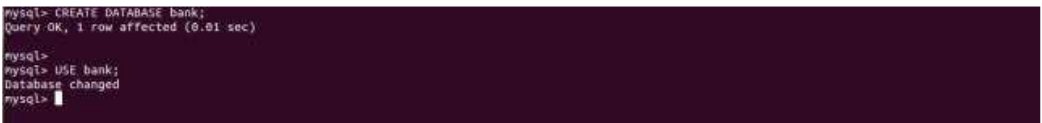
\includegraphics[width=12cm,height=3cm]{1.png}
    \caption{loan\_info}
\end{figure}
   \subsection{Creating table credit\_card\_info}
   CREATE TABLE credit\_card\_info \newline
( \newline
cc\_number bigint, \newline
user\_id int, \newline
maximum\_credit DOUBLE, \newline
outstanding\_balance DOUBLE, \newline
due\_date DATE \newline
); \newline
 
 \subsection{Inserting data into the credit\_card\_info table}
 insert into credit\_card\_info values(1234678753672899,1234,50000,35000,'2017-03-22');\newline insert
into credit\_card\_info values(1234678753672900,1243,500000,500000,'2017-03-12');\newline insert
into credit\_card\_info values(1234678753672902,1324,15000,12000,'2017-03-09');\newline insert into
credit\_card\_info values(1234678753672908,4312,60000,60000,'2017-02-16');\newline

\subsection{Checking the data in credit\_card\_info table}
select * from credit\_card\_info; \newline

\begin{figure}[H]
\centering
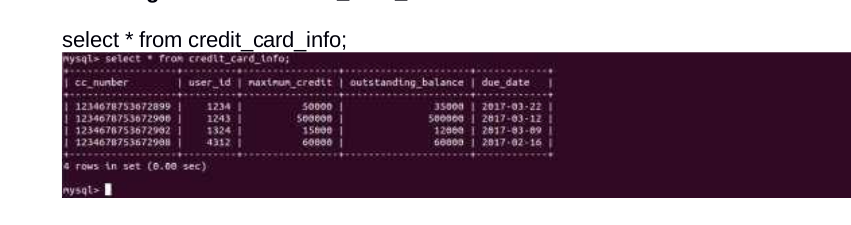
\includegraphics[width=12cm,height=3cm]{creditcard.png}
    \caption{creditcard\_info}
\end{figure}




\subsection{Creating table shares\_info}
CREATE TABLE shares\_info \newline
( \newline
share\_id varchar(10), \newline
company\_name varchar(20), \newline
gmt\_timestamp bigint, \newline
share\_price DOUBLE \newline
); \newline

\subsection{Inserting data into shares\_info table}
insert into shares\_info values('S102',"MyCorp",1488412702,100);\newline
insert into shares\_info values('S102',"MyCorp",1488411802,110);\newline
insert into shares\_info values('S102',"MyCorp",1488411902,90);\newline
insert into shares\_info values('S102',"MyCorp",1488412502,80);\newline
insert into shares\_info values('S102',"MyCorp",1488411502,120);\newline

\subsection{Checking the data in shares\_info table}
select * from shares\_info; \newline
commit; \newline

\begin{figure}[H]
\centering
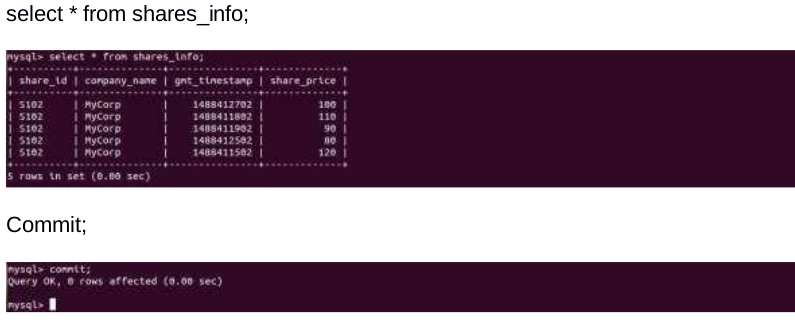
\includegraphics[width=12cm,height=3cm]{sharedinfor.png}
    \caption{shared\_info}
\end{figure}


\section{Exporting data from Mysql to HDFS using sqoop}

Now we have data in mysql. We need to export this data into HDFS. We will do it using sqoop.\newline
For exporting data into HDFS we will first create an user in mysql.\newline
CREATE USER 'myuser'@'localhost' IDENTIFIED BY \newline
'myuser'; grant all on *.* to 'myuser'@'localhost' with grant \newline
option; flush privileges; \newline
commit; \newline    
Now let's transfer these tables into HDFS by writing sqoop jobs.\newline
We will protect our mysql password by saving the password in a file.\newline
echo -n "myuser"\>>sqoop\_mysql\_passwrd\newline

You need to use the option -n. Otherwise, a new line will be created unknowingly and while \newline
reading the password, Sqoop throws an error Access Denied for User.\newline

/* \newline
Sqoop job to transfer data in loan\_info table \newline
Create a directory in HDFS loan\_info\_stg to store the table data \newline
hadoop fs -mkdir /bank \newline
hadoop fs -mkdir /bank/loan\_info\_stg \newline
Above step is not required while performing normal import. \newline
\subsection{Creating sqoop job for sqoop\_loan\_info}
sqoop job --create sqoop\_loan\_info -- import --connect \newline jdbc:mysql://localhost/bank \newline
--username \newline
myuser \newline
--table \newline
loan\_info  \newline
--password-file  \newline
file:///home/santosh/sqoop\_mysql\_passwrd --target-dir  \newline /bank/loan\_info\_stg -m1  \newline
sqoop job --list  \newline

\subsection{Executing the sqoop job sqoop\_loan\_info}

sqoop job --exec sqoop\_loan\_info \newline

Sqoop job to transfer data in credit\_card\_info table \newline

\subsection{Create a directory in HDFS for storing credit\_card\_info table data}

hadoop fs -mkdir /bank/credit\_card\_info\_stg

\subsection{Creating sqoop job credit\_card\_info}

sqoop job --create sqoop\_credit\_card\_info -- import --connect \newline
jdbc:mysql://localhost/bank -- \newline
username myuser --table credit\_card\_info --password-file\newline
\textbf{file:///home/santosh/sqoop\_mysql\_passwrd --target-dir /bank/credit\_card\_info\_stg -m} 1
sqoop job --list

\subsection{Executing the sqoop job sqoop\_loan\_info}
sqoop job --exec sqoop\_loan\_info

\subsection{Sqoop job to transfer data in shares\_info\_table}
\subsubsection{Creating HDFS directory to store shares\_info table data}
hadoop fs -mkdir /bank/shares\_info\_stg
\subsubsection{Creating sqoop job shares\_info}
sqoop job --create sqoop\_shares\_info -- myuser --table shares\_info --password-file \newline file:///home/santosh/sqoop\_mysql\_passwrd
/bank/shares\_info\_stg -m 1
sqoop job
\subsubsection{Executing sqoop\_job shares\_info}
sqoop job --exec sqoop\_shares\_info
--list
\section{Creating external tables in hive}
\subsection{Create database}
CREATE DATABASE bank; \newline
USE bank;
\subsection{Creating table loan\_info\_stg}
As this table is an external table, we just need to give the \newline location of the data.\newline
CREATE EXTERNAL TABLE loan\_info\_stg ( \newline
Loan\_id int,\newline
User\id int,\newline
last\_payment\_date string,\newline
payment\_installation double,\newline
Date\_payable string\newline
) ROW FORMAT DELIMITED FIELDS TERMINATED BY\newline
',' LOCATION '/bank/loan\_info\_stg';\newline

\subsection{Creating table credit\_card\_info\_stg}

CREATE EXTERNAL TABLE \newline
credit\_card\_info\_stg ( \newline
cc\_number string, \newline
user\_id int, \newline
maximum\_credit double, \newline
outstanding\_balance double, \newline
due\_date string \newline
) ROW FORMAT DELIMITED FIELDS TERMINATED BY \newline
',' LOCATION '/bank/credit\_card\_info\_stg'; \newline

\subsection{Creating table shares\_info\_stg}

CREATE EXTERNAL TABLE shares\_info\_stg \newline
( \newline
Share\_id string, \newline
Company\_name string, \newline
Gmt\_timestamp bigint, \newline
Share\_price double \newline
) ROW FORMAT DELIMITED FIELDS TERMINATED BY \newline
',' LOCATION '/bank/shares\_info\_stg'; \newline

\subsection{Creating core tables and loading the data into the core tables from stg tables}
Adding the udf into hive shell. \newline
CREATE TEMPORARY FUNCTION encrypt AS 'encryption.AESencrypt';\newline
CREATE TEMPORARY FUNCTION decrypt AS 'encryption.AESdecrypt';\newline
\subsection{Creating loan\_info table}
CREATE TABLE loan\_info ( \newline
Loan\_id string, \newline
User\_id string, \newline
last\_payment\_date string, \newline
payment\_installation string, \newline
Date\_payable string \newline
) STORED AS ORC; \newline

\subsection{Inserting data into loan\_info table}

INSERT INTO TABLE loan\_info \newline
SELECT encrypt(Loan\_id), \newline
encrypt(User\_id), \newline
encrypt(last\_payment\_date), \newline
encrypt(payment\_installation), \newline
encrypt(Date\_payable) \newline
FROM loan\_info\_stg; \newline

\subsection{Creating credit\_card\_info table}
CREATE TABLE credit\_card\_info \newline
( \newline
cc\_number string, \newline
user\_id string, \newline
maximum\_credit string, \newline
outstanding\_balance string, \newline
due\_date string \newline
) STORED AS ORC; \newline

\subsection{Inserting data into credit\_card\_info table}
INSERT INTO TABLE credit\_card\_info \newline
SELECT encrypt(cc\_number), \newline
encrypt(User\_id), \newline
encrypt(maximum\_credit), \newline
encrypt(outstanding\_balance), \newline
encrypt(due\_date) \newline
FROM credit\_card\_info\_stg; \newline

\subsection{Creating shares\_info table}
CREATE TABLE shares\_info \newline
( \newline
Share\_id string, \newline
Company\_name string, \newline
Gmt\_timestamp string, \newline
Share\_price string \newline
) STORED AS ORC;\newline

\subsection{Inserting data into shares\_info table}
INSERT INTO TABLE shares\_info \newline
SELECT encrypt(Share\_id), \newline
encrypt(Company\_name), \newline
encrypt(Gmt\_timestamp), \newline
encrypt(Share\\price) \newline
FROM shares\_info\_stg; \newline

\subsection{Checking the data in the three tables}
As the data is bank data, we have encrypted the data.\newline
You can truncate the data from stg tables.\newline

\section{Analysis}
\subsection{Decrypting the data for analysis}
CREATE TEMPORARY FUNCTION encrypt AS 'encryption.AESencrypt';\newline
CREATE TEMPORARY FUNCTION decrypt AS 'encryption.AESdecrypt';\newline
CREATE TEMPORARY FUNCTION max\_profit AS 'maxprofit.MaxProfit';\newline
SET hive.auto.convert.join=false;\newline

\subsection{Find out the list of users who have at least 2 loan instalments pending.}
SELECT decrypt(user\_id) \newline
FROM loa\_info \newline
WHERE datediff(from\_unixtime(unix\_timestamp(), 'yyyy-MM-dd'), \newline
decrypt(last\_payment\_date)) >= 60; \newline

\subsection{Find the list of users who have a healthy credit card but outstanding loan account.
Healthy credit card means no outstanding balance.}
SELECT decrypt(li.user\_id) \newline
FROM loan\_info li INNER JOIN credit\_card\_info \newline
cci ON decrypt(li.user\_id) = decrypt(cci.user\_id) \newline
WHERE CAST(decrypt(cci.outstanding\_balance) AS double) = 0.0 \newline
AND datediff(from\_unixtime(unix\_timestamp(), 'yyyy-MM-dd'), \newline
decrypt(li.last\_payment\_date) >= 30); \newpage

\subsection{For every share and for every date, find the maximum profit one could have made
on the share. Bear in mind that a share purchase must be before share sell and if share
prices fall throughout the day, maximum possible profit may be negative.}
\begin{verbatim}
SELECT share_id, share_date,
max\profit(collect_list(share_price))
FROM
( 
SELECT decrypt(Share_id) AS share_id,
decrypt(Gmt_timestamp) AS Gmt_timestamp,
from_unixtime(CAST(decrypt(Gmt_timestamp) AS int), 'yyyy-MM-dd')
share_date, CAST (decrypt(Share_price) AS double) AS share_price FROM
shares_info
DISTRIBUTE BY share_id,
from_unixtime(CAST(Gmt_timestamp AS int), 'yyyy-MM-dd')
SORT BY share_id,
CAST(Gmt_timestamp AS int)
) inne GROUP BY share_id, share_date;
\end{verbatim}
\section{Survey data analysis}

We have 3 survery part files. So we will copy the contents into a \newline single file using the below \newline
linux commands. \newline
cd /home/acadgild/survey\_files \newline
cat *.txt > survey\_data \newline
rm *.txt \newline
Now we have the concated data in survey\_data file.\newline
\newpage
\subsection{Creating hive table to load survey\_data}

CREATE TABLE survey\_analysis ( \newline
survey\_date string, \newline
survey\_question string, \newline
Rating int, \newline
user\_id int, \newline
survey\_id string \newline
) \newline
ROW FORMAT DELIMITED  \newline
FIELDS TERMINATED BY ',';  \newline

\subsection{Loading data into survey\_analysis table}

LOAD DATA LOCAL INPATH '/home/acadgild/survey\_files/survey\_data'\newline INTO TABLE \newline
bank.survey\_analysis; \newpage


\section{Result}
\begin{itemize}
    \item The localhost page of Hadoop is shown in figure 16.To access this page, step to be followed:\\
Start Hadoop services form terminal.\\
Enter localhost:50070 in web address of any web browser.\\
from this page user can browse the file system.
\end{itemize}
\begin{figure}[htb]
\centering
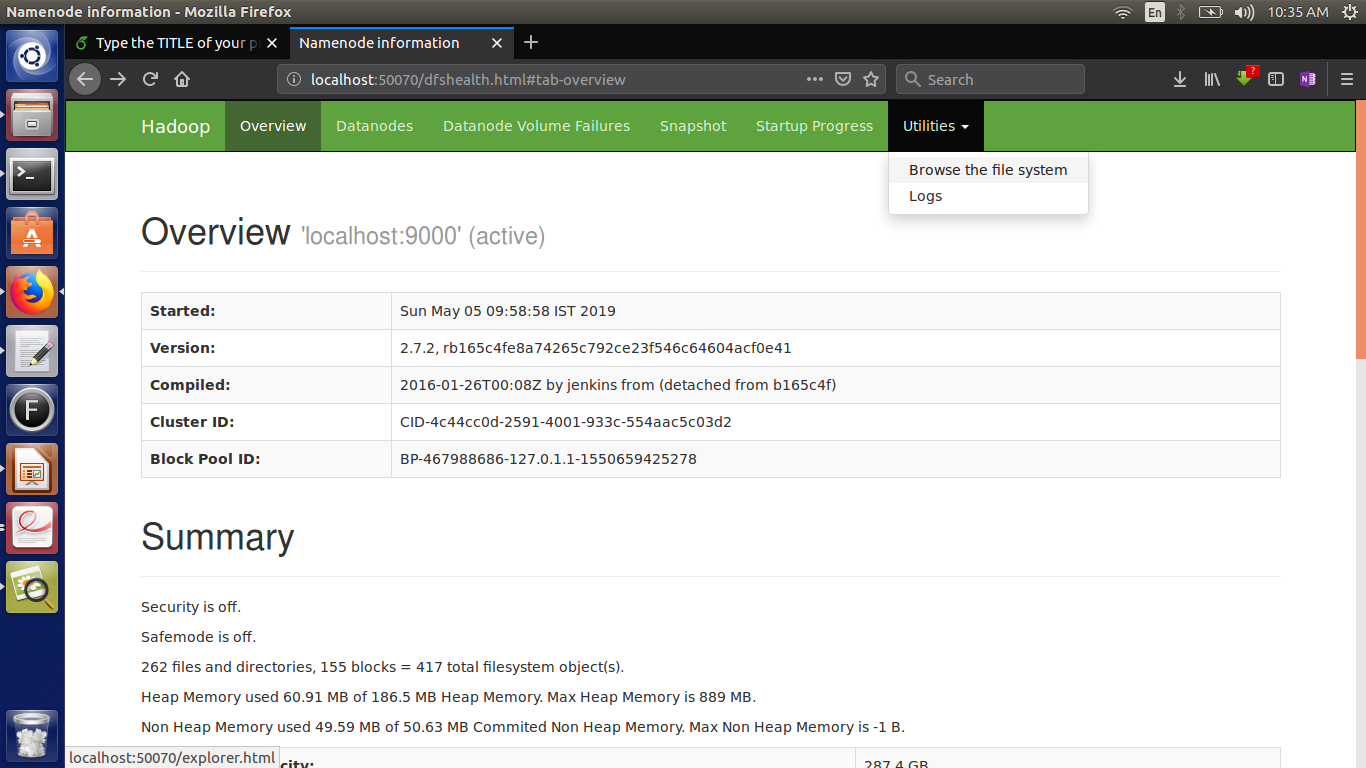
\includegraphics[width=8cm,height=8cm]{1stp.png}
    \caption{Browsing File}
\end{figure} \newpage
\begin{itemize}
    
\item  From browse the file system, User can view screen as shown in figure 17. Now ,User can select Bank related to detail he/she have stored,

\end{itemize}
\begin{figure}[htb]
\centering
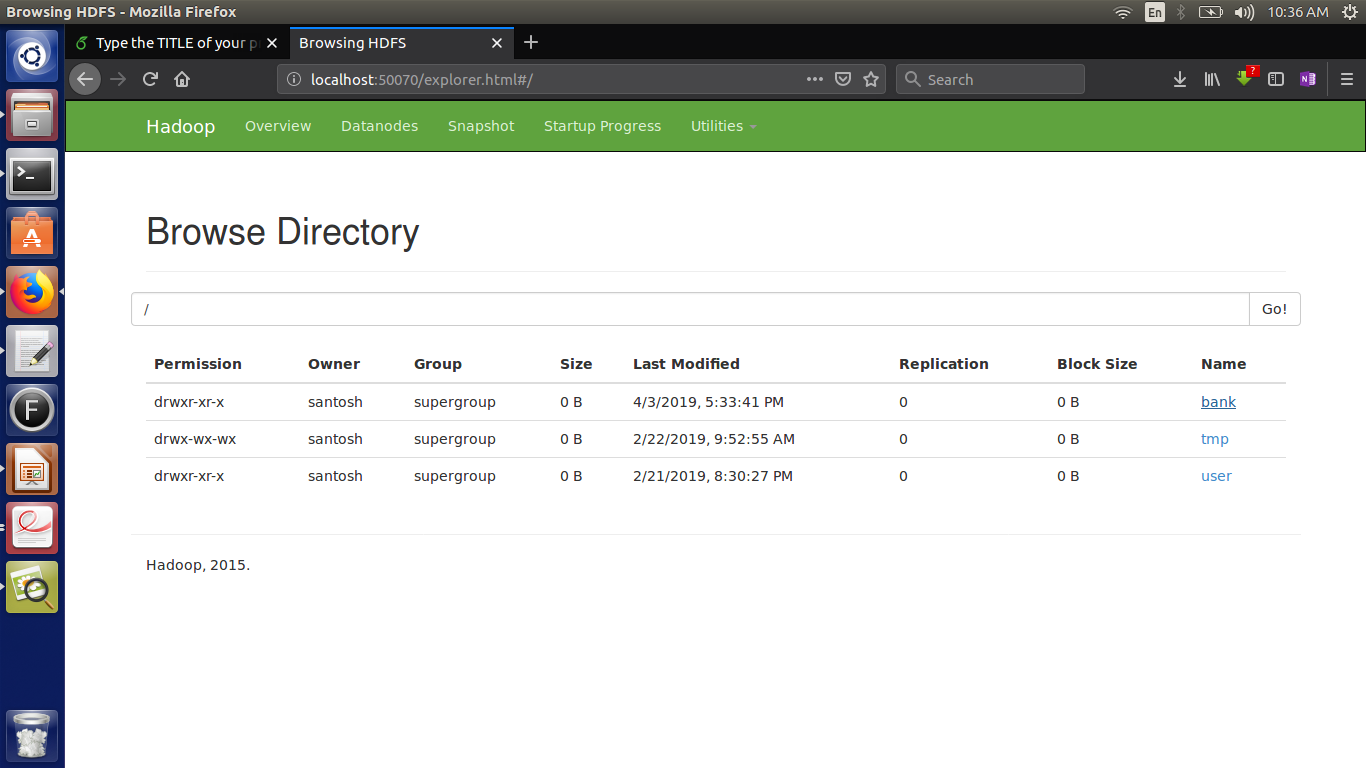
\includegraphics[width=8cm,height=8cm]{2ndp.png}
    \caption{Bank information}
\end{figure} \newpage
\begin{itemize}
    \item 

This diagram represent Credit Card Information means that a credit card is different from a charge card, which requires the balance to be repaid in full each month.In contrast, credit cards allow the consumers to build a continuing balance of debt, subject to interest being charged. A credit card also differs from a cash card, which can be used like currency by the owner of the card. A credit card differs from a charge card also in that a credit card typically involves a third-party entity that pays the seller and is reimbursed by the buyer, whereas a charge card simply defers payment by the buyer until a later date.
\end{itemize}
\begin{figure}[htb]
\centering
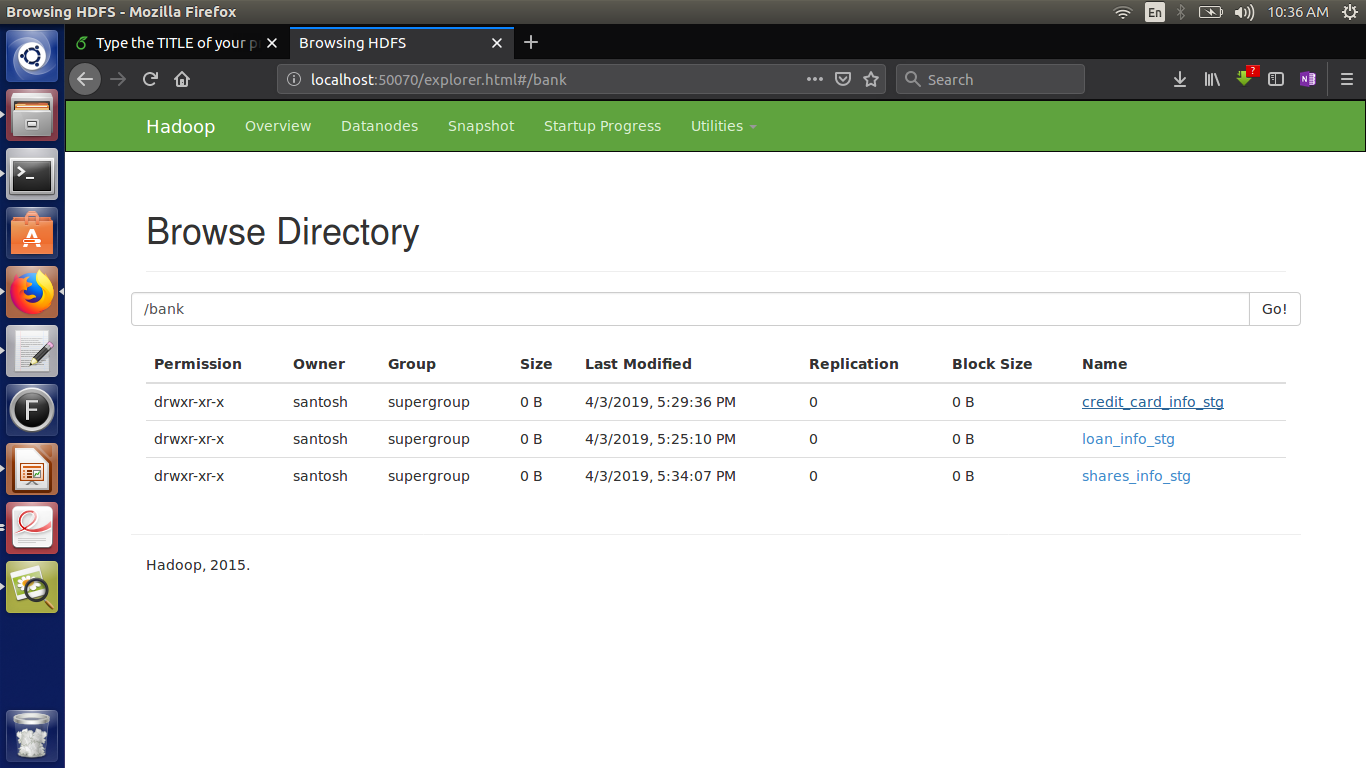
\includegraphics[width=8cm,height=8cm]{3p.png}
    \caption{credit card information}
\end{figure} \newpage
\begin{itemize}
    \item The Credit card information is successfully uploaded.

 
 \end{itemize}
\begin{figure}[htb]
\centering
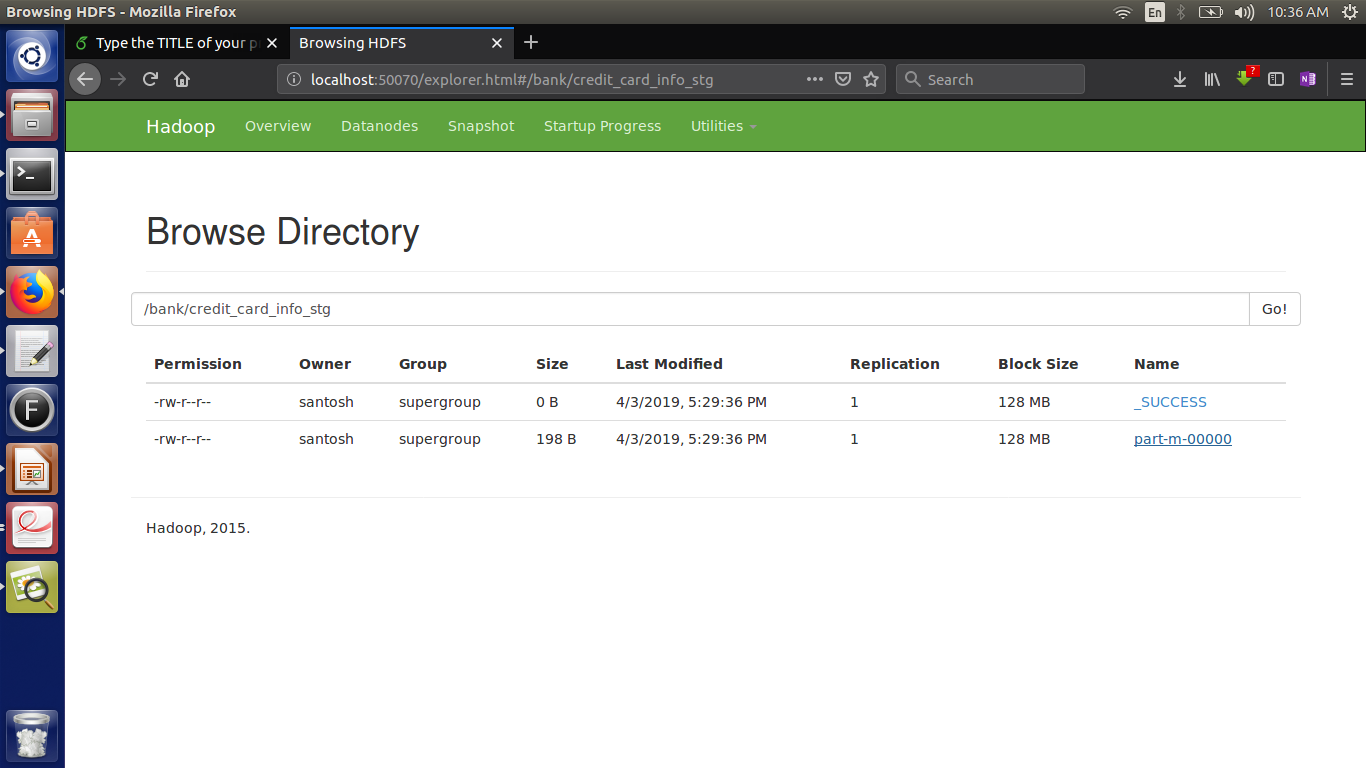
\includegraphics[width=8cm,height=8cm]{4p.png}
    \caption{Browsing Data}
\end{figure} \newpage
\begin{itemize}
    \item After selecting credit card information link user can download data using screen link. This related page is as shown in figure.
\end{itemize}
\begin{figure}[htb]
\centering
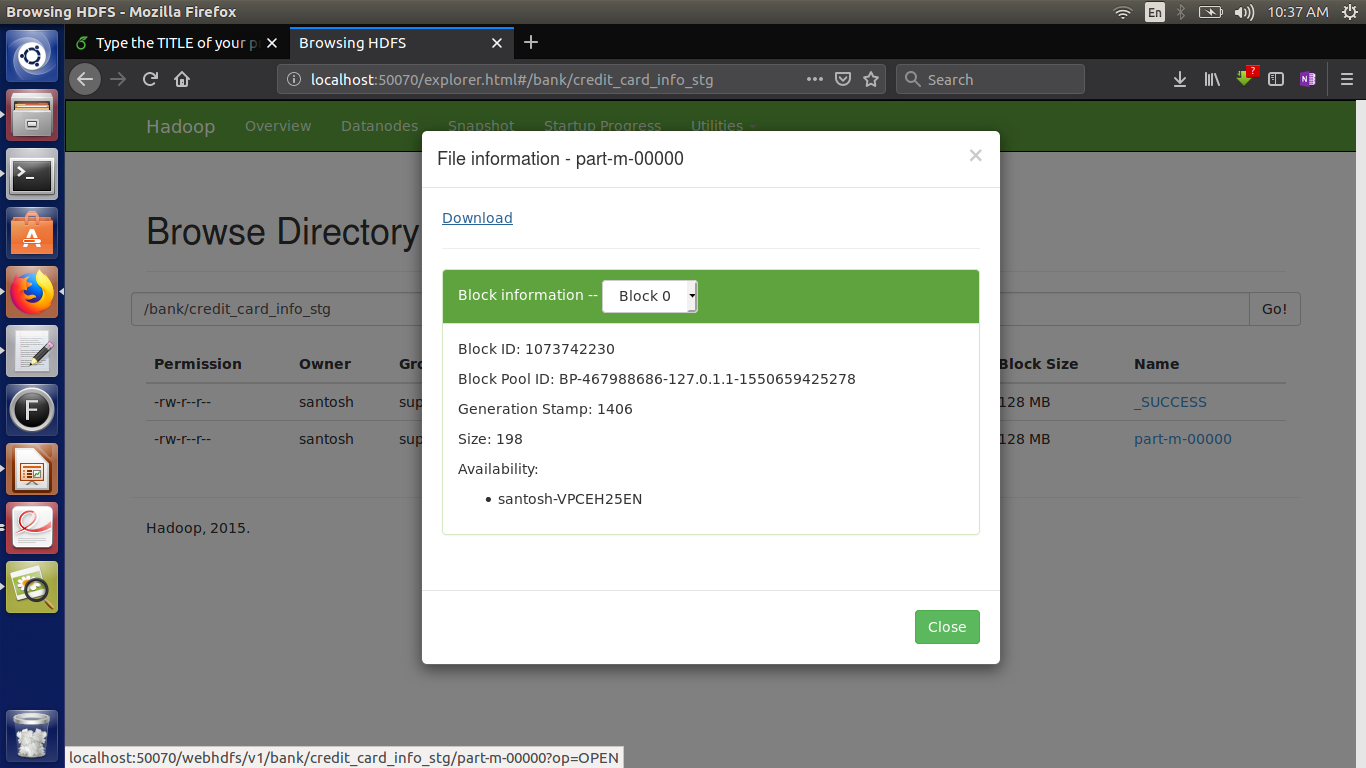
\includegraphics[width=8cm,height=8cm]{5p.png}
    \caption{File Information}
\end{figure} \newpage
\begin{itemize}
    \item After selecting loan information link form Bank, User can download data using success link. the related page is shown in figure.
    \item A loan is the lending of money by one or more individuals, organizations, or other entities to other individuals, organizations etc. The recipient (i.e. the borrower) incurs a debt, and is usually liable to pay interest on that debt until it is repaid, and also to repay the principal amount borrowed. 
\end{itemize}
\begin{figure}[htb]
\centering
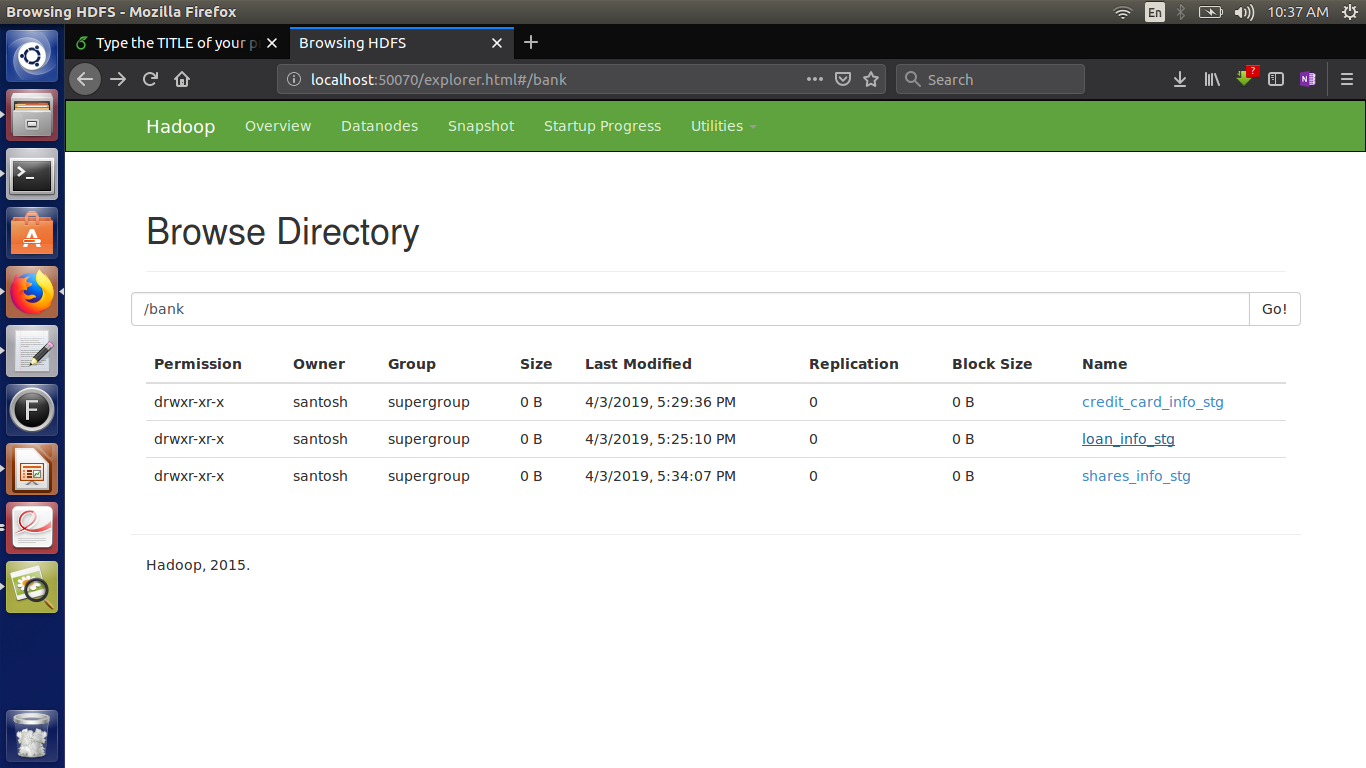
\includegraphics[width=8cm,height=8cm]{6p.png}
    \caption{loan Information}
\end{figure} \newpage

\begin{itemize}
    \item In this section all the data have successfully update.
\end{itemize}
\begin{figure}[htb]
\centering
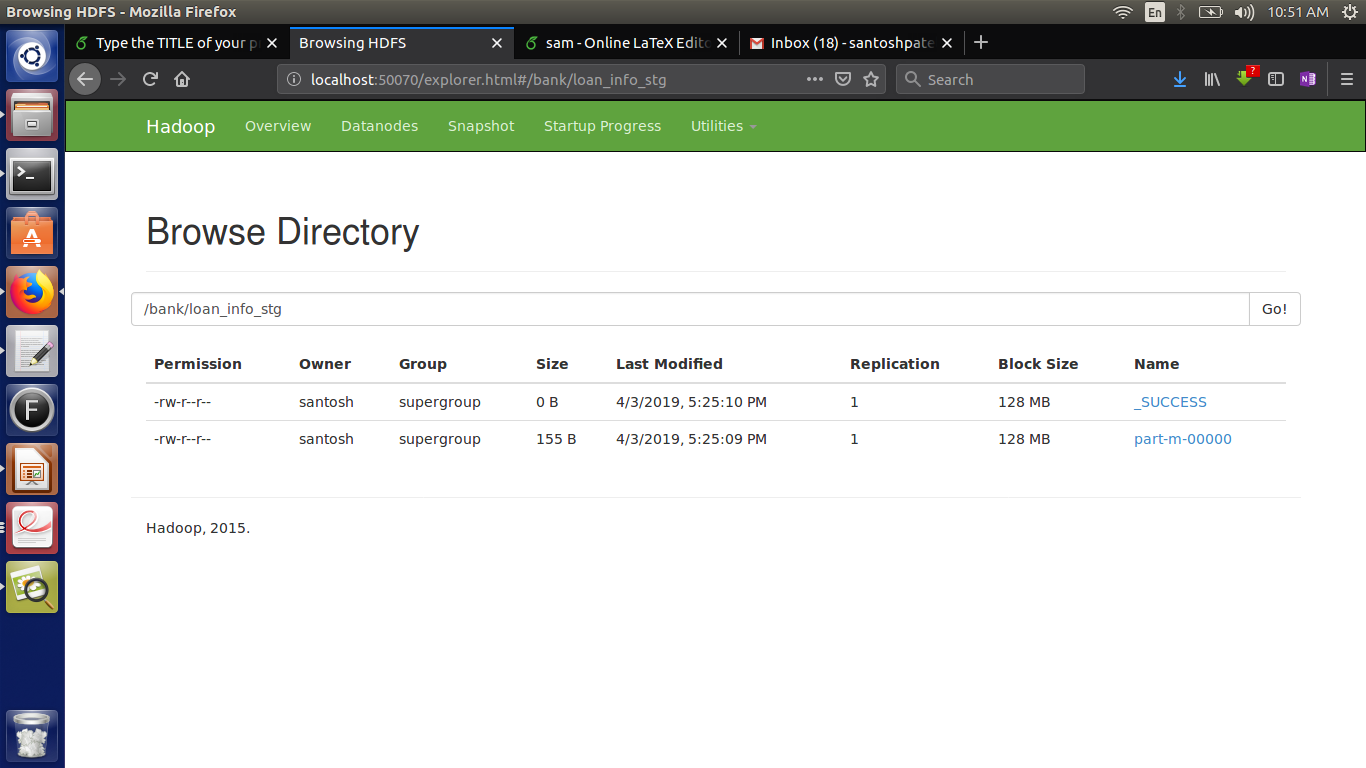
\includegraphics[width=8cm,height=8cm]{7pag.png}
    \caption{File information of loan}
\end{figure} \newpage

\begin{itemize}
    \item The download link appears as shown in figure.
\end{itemize}
\begin{figure}[htb]
\centering
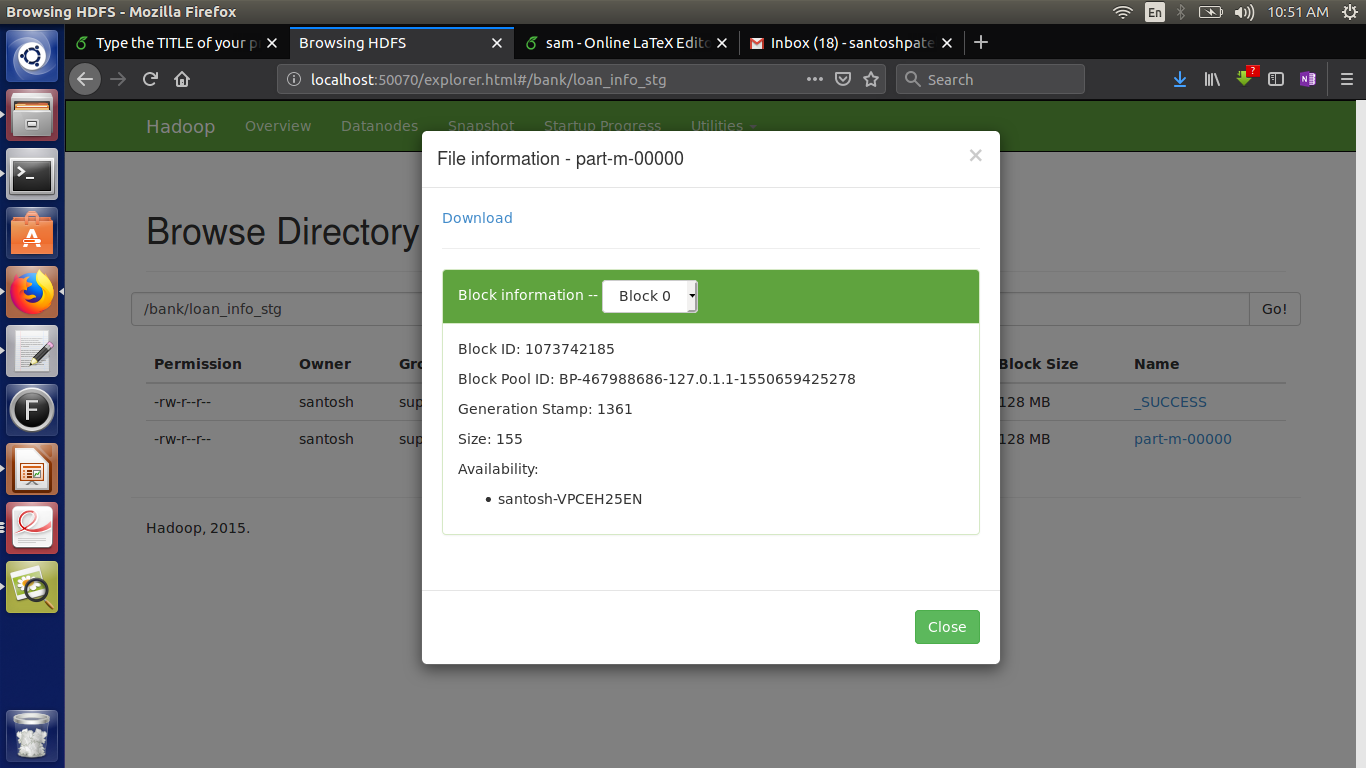
\includegraphics[width=8cm,height=8cm]{8page.png}
    \caption{Browsing File}
\end{figure} \newpage
\begin{itemize}
    \item After the selecting shares information link, User can download data using success link.the related page is shown in figure.
\end{itemize}

\begin{figure}[htb]
\centering
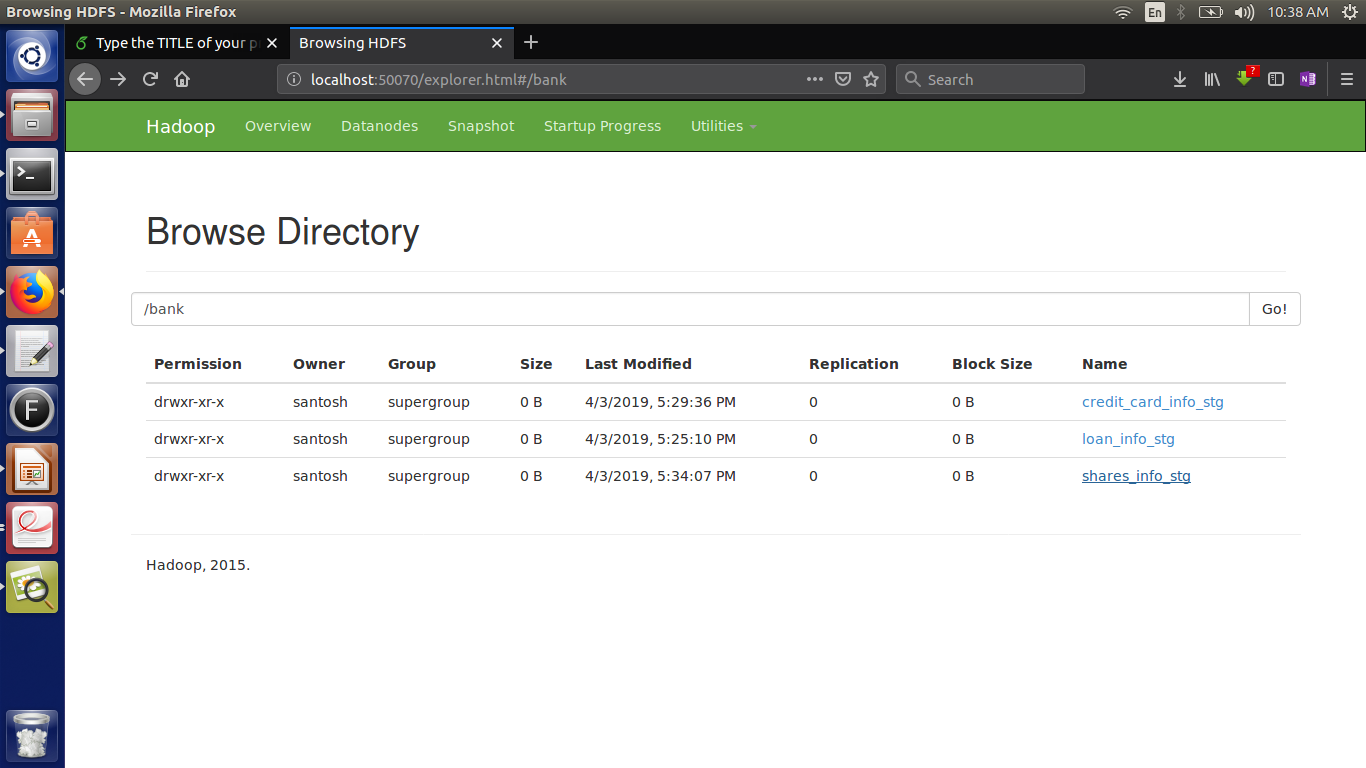
\includegraphics[width=8cm,height=8cm]{9thp.png}
    \caption{Browsing File shares information}
\end{figure} \newpage
\\

\begin{itemize}
    \item All data have been successfully upload.
\end{itemize}
\begin{figure}[htb]
\centering
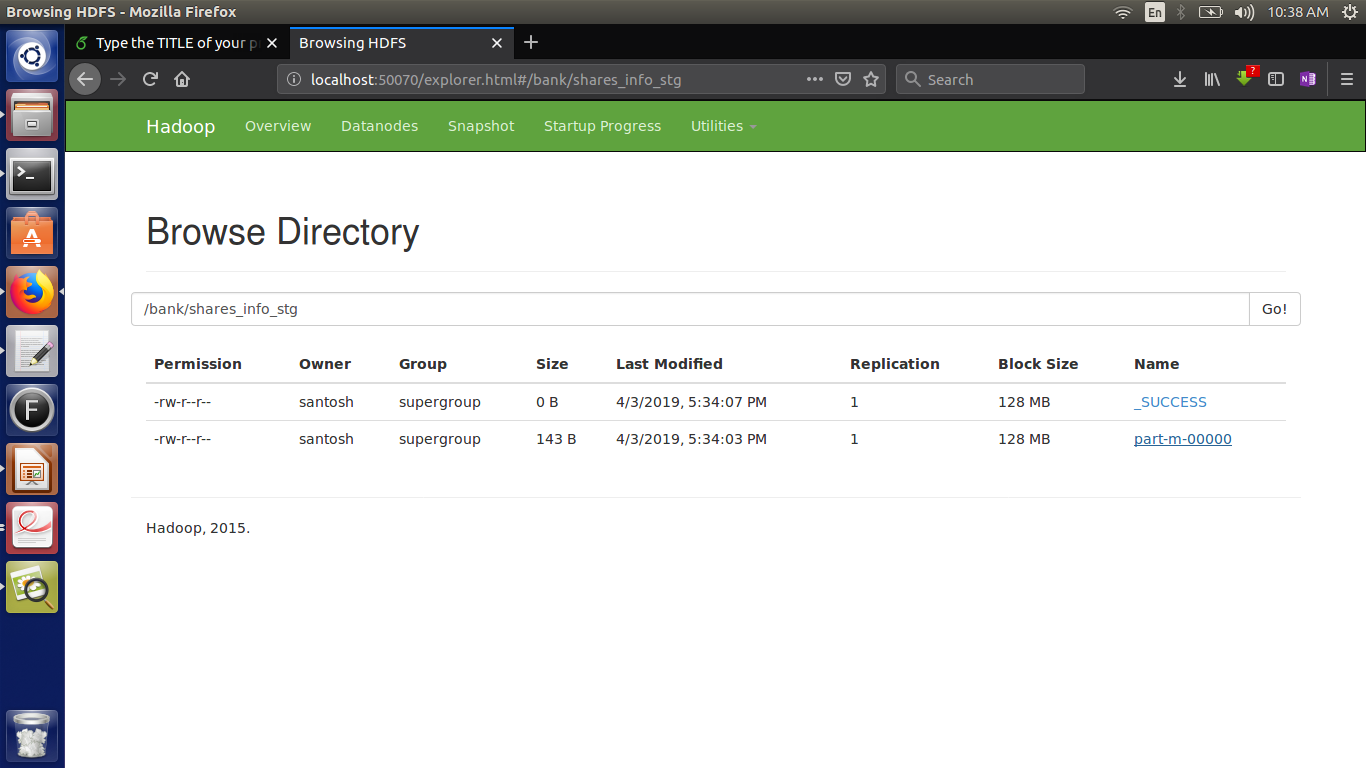
\includegraphics[width=8cm,height=8cm]{10p.png}
    \caption{shares information}
\end{figure} \newpage



\flushbottom

\flushbottom
\include{chapter4}
\flushbottom

\flushbottom
\chapter{Conclusion and Future Work}
\subsection{Conclusion}
Bank are creating large amount of data day by day. Their creation speed is much faster than our processor's speed.So the handling of bulk amount of data is difficult for our system. But storing and processing of Big Data is faster when it stored in distributed manner. Hadoop framework provides such king of network where Big Data distributed among different system.By adding more nodes.Data can be store in different in different location.If any nodes fails then there is no loss of data.By the use of big data banks run more profitably. To make money, banks use deposits and whole sale deposits, share equity and fees and interest from debt, loans and consumer lending, such as credit cards and bank fees. History has proven banks to be vulnerable to many risks, however, including credit, liquidity, market, operating, interesting rate and legal risks.\newpage
\subsection{Future Work}
Hardware and Software can be minimize so that user base can increase.\newline
Working process can reduced so that efficiency and performance of the application can improve.\newline
To ensure that data analytics future is great in India, normal development & use of big data subsequently must be supported to boost scope of Data Analytics. Banks use data mining methods to filter the populated data. 
\flushbottom

\flushbottom
\include{chapter6}
\flushbottom






\begin{thebibliography}{8}

\bibitem{cc}
Introduction to Big Data Analytics:A Webinar by Wizlq Education. 
\bibitem{lan}
Big Data analytics using Hadoop: A Lecture by Durga Software Solution.
\bibitem{com}
Book Followed:\newline
Information technology for management by Efraim Turban,Linda Volonino.\newline
Data Analytics Made Accessible, by A. Maheshwari.

\bibitem{car}
Website Followed:https://www.flysas.com
\bibitem{com2}
https://www.smartdatacollective.com


\end{thebibliography}


\appendix
\chapter{Biographical Sketch}
\begin{center}
\textbf{\large Santosh Kumar}\par
At-Devdan, P.O-Chhardhi, Ps-Kalwari,Dist-Basti, State-Uttar Pradesh, Pin-272301\\
 Email-santoshpatel.nita@gmail.com, Contact No.-9565925350 
\end{center}
\begin{enumerate}
  % \item[$cdot$ bla1] item 1
  \item[$\bullet$] Pursuing MCA, From National Institute of Technology, Agartala with CGPA of 7.01/10.
	\item[$\bullet$]B.Sc from K.S.Saket P.G. college Ayodhya Faizabad, Uttar Pradesh with 63.33 \% in 2015.
	\item[$\bullet$]Intermediate from B.P.R.K.I.C Khoria Bazar Basti, Uttar Pradesh with 60.00 \% in 2012.
	\item[$\bullet$]10\textsuperscript(th) from Raghuraj Ram Tiwari HSS Gaighat Basti, Uttar Pradesh with 55.00 \% in 2010.
\end{enumerate}
\end{document}